\newcommand{\cupdot}{\mathbin{\mathaccent\cdot\cup}}

\chapter{Верхние и нижние оценки}
\label{chapter3}

%По-моему, повтор первой главы. 
%И вообще, не здесь нужно говорить об оценках, а во второй главе. Зедсь чуть-чуть расписать про операторы и погнать примеры.

\section{Оценка сложности алгоритмов с несмещенными операторами}

Особый интерес в рамках данной работы над задачей Needle представляет собой класс несмещенных алгоритмов арностей $k$. Под несмещенными алгоритмами (произвольной арности) понимаются алгоритмы
следующего вида:

\begin{itemize}
   \item Запрос $Q_1$ - запрос, сгенерированный случайным образом.
   \item Запрос $Q_{i+1}$ - реализация случайной величины, такой что:
    $ \forall z: p(Q_{i+1} | Q_1, ... Q_i, A_1, ... A_i) =  
     p(Q_{i+1} \oplus z | Q_1 \oplus z, ..., Q_i \oplus z, A_1, ..., A_i) $
    \begin{align*}
    \forall perm():  p(Q_{i+1} | Q_1, ..., & Q_i, A_1, ..., A_i) = \\ &= p(perm(Q_{i+1}) |perm(Q_1), ..., perm(Q_i), A_1, ... A_i) 
    \end{align*}
  \end{itemize}
         
Иными словами, функция, генерирующая запрос, не меняется, если индексы всех битовых строк переставить одинаковым образом, или если все битовые строки поксорить с константой. 

Алгоритм арности $k$: случайная величина, генерирующая $Q_{i+1}$ рандомизировано выбирает не более k различных индексов $H_j$ из $[1; i]$ и генерирует $Q_{i+1}$ используя только 
$Q_{H_1}, \ldots, Q_{H_K}, A_{H_1}, \ldots A_{H_K}$. Разумеется, при этом она обязана быть несмещенной.

Для примера, унарный ($k = 1$) алгоритм может следующий запрос сделать либо совсем случайным, либо взять какой-то из предыдущих запросов и применить к нему унарный несмещенный <<оператор мутации>>. 
Унарные операторы мутации, как нетрудно показать, имеют вид <<выбрать из некоторого распределения число $X$ (от 0 до $n$), выбрать случайным образом $X$ различных битовых индексов и перевернуть биты на 
каждом из этих индексов>>.

Особый интерес представляют собой несмещенные операторы арностей $k = 1, 2, 3$, а соответственно и несмещенные алгоритмы, работающие с данными операторами.

В рамках рассматриваемой black-box сложности, получение оценок на сложность работы алгоритмов состоит в нахождение верхних и нижних оценок. 
Верхние оценки сложности представлют собой оценку работы некоторого алгоритма, который решает задачу. При этом алгоритм не обязательно является эволюционным. 
Верхняя оценка~--- оценка любого алгоритма, решающего задачу в принципе. 

Нижние оценки представляются гораздо сложнее. Чаще всего для получения нижних оценок используются информационно-теоретические оценки, что гораздо сложнее, чем получение верхних оценок. 
Зачастую подсчет сводится к нахождению общего вида всех алгоритмов данного класса, нахождению вещественнозначных параметров, однозначное определяющих работу алгоритма, построению выражения, 
зависящего от указанных параметров и определяющего математическое ожидание времени работы алгоритма, и, наконец, минимизации времени работы. При отсутствии аналитического решения задача 
решается численным моделированием.   

\subsection{Тернарный алгоритм}
\label{ternary}

%бедно и непонятно, исправить обязательно. Может подумать о картинке в пример, дабы было нагляднее. 


В качеcтве операторов для данного алгоритма введем следующие несмещенные операторы: 
\begin{itemize}
   \item $flipOne(a)$ - изменение одного бита
   \item $flip'(a, b)$ - изменить один бит из совпадающего суффикса
   \item $xor3(a,b,c)$ - оператор исключающего ИЛИ для трех векторов 
\end{itemize}

(вставить формальное доказательство, что xor3 -> несмещенный)

Тогда рассмотрим следующий алгоритм: 
\begin{algorithm}[H]
\caption{Тернарный алгоритм}\label{lst1}
\begin{algorithmic}
        \State $q_0$ \leftarrow $\textrm{random}$ \\
        \State $s_1$ \leftarrow $flipOne(q_0)$
		\While{true}
	        \State $s_2$ \leftarrow $flip'(q_0, s_1)$
            \State $t_2$ \leftarrow $xor3(q_0,s_1,s_2)$
            \State $s_3$ \leftarrow $flip'(q_0, t_2)$
            \State $t_3$ \leftarrow $xor3(q_0,s_2,s_3)$
            \State ...
		\EndWhile
\end{algorithmic}
\end{algorithm}

Таким образом формируется полное пространство поиска: 
\begin{example}
Пример генерации пространства для q_0 = [000...000]  \\
\end{example}

\begin{figure}[H]
%\caption{Пример генерации множества поиска для q0}\label{fig2}
    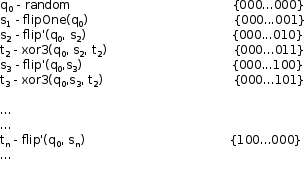
\includegraphics[height=7cm]{ITMO/pic/tern0.png}
\end{figure}


%Размазано и непонятно. Переписать точно.
Таким образом пошагово генерируется все множество поиска без повторов. Сложность такого алгоритма равняется O($\frac{2^n + 1}{2}$), что равняется времени перебора всех векторов без повторов. Таким образом, верхняя и нижняя оценки сложности алгоритма совпадают. 


%Что-то вроде примера 
Рассмотрим класс некоторых задач, таких что экземпляром данной задачи является битовая строка из пространства поиска, размера $2^n$ от длины строки n. При этом у задачи существует единственный глобальный оптимум (при этом  наличие других оптимумов не важно). К таким задачам относится, например, OneMax.

Задачи данного класса должны имееть примерно такой тип:
$$P = \{..2^n \textrm{instanses with bitwise} ... \}$$

Пусть существует оптимальный детерминированный алгоритм, который в среднем по всем экзеплярам выдает время работы T, при этом алгоритм не является black-box алгоритмом. 

Пусть $q_0$ - рандомизированный вектор, подающийся на вход алгоритму.

Тогда дерево решений данного алгоритма выглядит так: 

\begin{figure}[H]
\caption{Дерево решений детерминированного алгоритма}\label{fig2}
    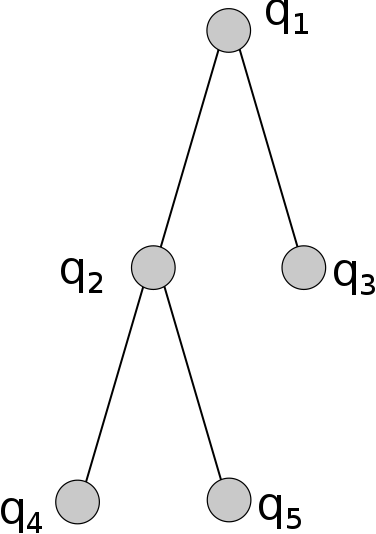
\includegraphics[height=5cm]{ITMO/pic/graph1.png}
\end{figure}

Возьмем произвольный вектор z и проксорим его с каждым решением из приведенного выше дерева. Таким образом все равно получится оптимальный детерминированны алгоритм, решающий данную задачу, но выглядеть он будет уже иначе, допустим, так: 

\begin{figure}[H]
\caption{Дерево решений другого оптимального алгоритма}\label{fig2}
    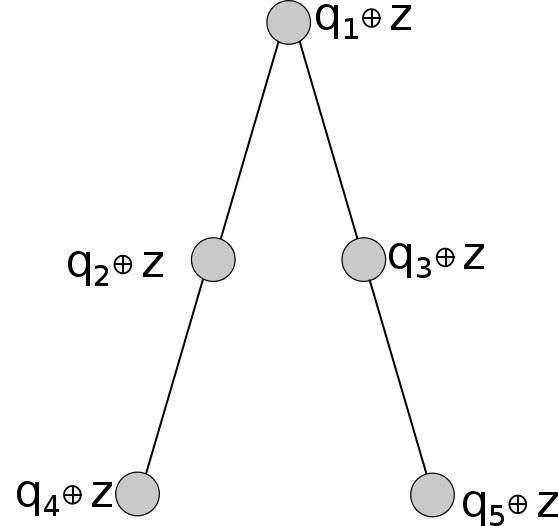
\includegraphics[height=5cm]{ITMO/pic/graph2.png}
\end{figure}

Тогда моделизируем процесс. 
$q_0$ - так и остается рандомизированным вектором.
Исходя из дерева решений, известно, что переход в дереве от $q_1 \to q_2$ является не более чем изменением одного бита. 

Так как при моделировании аллгоритма с тернарным оператором мы можем сгенерировать множество векторов, показанное в примере 3, то мы умеем получать переходы при изменении от одного бита к другому. 

Тогда z больше не просто случайный вектор, а $z = q_0 \oplus q_1 $, что, таким образом, и будет являться переходом $q_1 \to q_2$ в дереве решений. А так как при применения $\oplus$ к вершине изначального дерева, так же получается детерминированный алгоритм, то учитывая построение множества, тогда несмщенный black-box алгоритм будет работать за $\leq(n + 1)T$



\subsection{Бинарный алгоритм}
\label{binary}

Основная идея алгоритма с несмещенныи бинарными операторами заключается в следующих двух этапах: формирование независимых уникальных строк без использования операторов 
с помощью примитивных пошаговых пеобразований и формирование всего оставшегося множества поиска, стараясь минимизировать количество повторений. 

Рассмотрим первый этап: создание множества уникальных строк.

Введем следующее: пусть ${I_0}^1 = \{1,\ldots, n\}$ - множество индексов в искомом экземпляре, поданном на вход задаче. 

Каждый этап выглядит следующим образом: 
\begin{align*}
& L_i = \langle \mathcal{I}_i = \{{\mathcal{I}_{i}}^{1},....{\mathcal{I}_{i}}^{k};\}; \:\: \textrm{где}  \cupdot_{a = 1..k_i} {I_i}^a = \{ 1..n \}; \\
& S_i = \{ {S_i}^1, ... {S_i}^{m_i}, \}, \textrm{где}  \\ 
&{s_i}^j = b_1..b_{k_i}, b_k = \{ 0..1  \}  \Longleftrightarrow b_1 \textrm{ на индексах } {I_{i}}^1, \\ & \:\:\:\:\:\:\:\:\:\:\:\:\:\:\:\:\:\:\:\:\:\:\:\:\:\:\:\:\:\:\:\:\:\:\:\:\:\:\:\:\:\:\:\:\:\:\:\:\:\:\:\:\:\:\:\: b_e \textrm{ на индексах } {I_{i}}^e\\
 \rangle
\end{align*}

Таким образом, самый первый уровень будет выглядеть так: 
$$L_0 = \langle \{\{ 1...n \}\}, \{0\} \rangle.$$

Каждый последующий уровень $L_i$ можно получить двумя способами: 
\begin{itemize}
   \item Разделить одно из множеств индексов пополам: $ \mathcal{{I}_i}^j \to \{\mathcal{{I}_{i+1}}^j, \mathcal{{I}_{i+1}}^{k_i+1}\} $, где $j \in [1..k_i]$;
   \item Преобразование строк с помощью операций, не разрезающих множества индексов.
\end{itemize}

При разделении множества индексов, уже имеющиеся строки преобразуются удваиванием бита, находящегося на позиции, множество индексов которого разделилось.
Таким образом гарантируется, что следующая полученная строка будет уникальна.

К неразделяющим множества индексов операциям относятся следующие оперции, которые можно применять попарно ко всем полученным векторам: 
переворот несовпадающих бит, переворот совпадающих бит, поворот совпадающих и несовпадающих бит. 
Нетрудно заметить, что данные операции являются несмещенными, так как не ориентируются на положение бита, а только на совпадение в этой же позиции с битом второго вектора. 

Таким образом генерируются маски последуюших строк. 

\begin{example}
Пример генерации строк для вектора размера $n = 6$ \\
    I = \{1, 2, 3,4,5,6\} \:\: S = \{0\} \\
    I = \{1, 2, 3,4,5,6\}  \:\: S = \{0, 1\} \\
    I = \{1, 2, 3\}, \{4,5,6\} \:\: S = \{00, 11\} \\
    I = \{1, 2, 3\}, \{4,5,6\} \:\: S = \{00, 11, 01, 10\} \\
    I = \{1, 2\}, \{3\}, \{4,5,6\} \:\: S = \{000, 111, 001, 110\} \\
    I = \{1, 2\}, \{3\}, \{4,5,6\} \:\: S = \{000, 111, 001, 110, 011, 100\} \\
    ...
\end{example}

В силу перечисленных выше изменений векторов, из полученных масок и индексов генерируется некоторое число уникальных строк. 
Так как таким путем нельзя получить полное множество поиска, оставшиеся строки генерируются следующим образом:  

\begin{algorithm}[!h]
\caption{Black-box алгоритм в несмещенной модели}\label{lst1}
\begin{algorithmic}
		\For{$t = S_1,S_2,S_3,...,S_\phi$ }
	    \State choose $i \in [1 : \phi] $
	    \State choose $j \in [1 : \phi] $
	    \State $e \leftarrow$ same bits in $\{S_i, S_j\}$
	    \State $d \leftarrow$ different bits in $\{S_i, S_j\}$
	    \State choose $k \in [1 : e] $
	    \State choose $l \in [1 : e] $
	    \State add to $T_{ijkl}$ - множество строк, генерируемых из $S_i$ и $S_j$ путем инвертирования k совпадающих и l различающихся бит в $S_i$
		\EndFor
\end{algorithmic}
\end{algorithm}

Таким образом генерируется множество конструкций, содержащих $T_{ijkl}$:   $\mathbb{T} = \{ T_{ijkl} \}$.
    
    \begin{math}
        \mathbb{T'} \subseteq \mathbb{T} : 
                   \left\{  
           \begin{array}{rcl}  
            \forall t, u \in \mathbb{T'} \quad t \cap u = \varnothing \\  
              \cup = {\{0, 1 \}}^n \setminus \{S_1...S_{\phi}\} \\  
           \end{array}   
           \right.
    \end{math}


Таким образом, мы получаем область поиска с некоторыми повторами, что немного, но улучшает работу. С увеличением длины подаваемого на вход вектора, увеличивается количество повторов.
На рисунке~\ref{fig1} показано распределение множества $T'$ для $n = 6$. При этом размер множества составлял 4097 строк.

\begin{figure}[H]
\centering
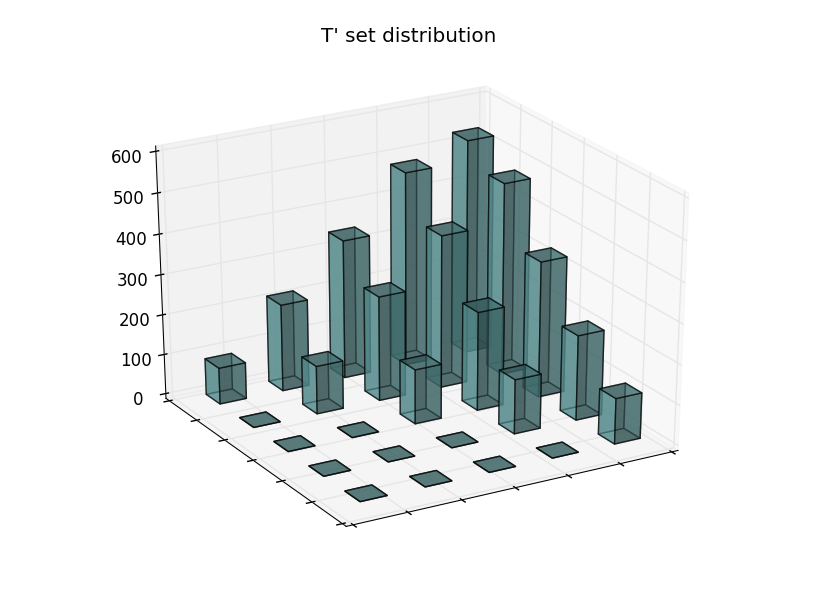
\includegraphics[height=10cm]{pic/fig6_n.png}
\caption{Распределение для n = 6}\label{fig1}
\end{figure}

Для улучшения результатов, применим к получившемся множествам некоторые преобразования. Сравним некоторые множества $T_{ijkl}$ между собой на наличие повторяющихся строк следующим образом: 

\begin{algorithm}[H]
\caption{Фильтрация повторяющихся множеств}\label{lst1}
\begin{algorithmic}
        \State Создаем неориентированный граф, вершины которого - множества $T_{ijkl}$ 
        \For{$i = 0, 1, \ldots, \mathbb{T}.same$}
	        \For{$j = 0, 1, \ldots, \mathbb{T}.diff$}
    	        \State Если между двумя множествами нет совпадающих строк, то соединяем данные вершины ребром.   
	        \EndFor
	    \EndFor
	    \State Дальнейшая задача сводится к поиску максимальной клики в графе.
\end{algorithmic}
\end{algorithm} 

По результатам работы алгоритма были рассмотрены два варианта действий. 
Рассмотрим несколько максимальных полученных клик, множества которых покрывают все пространство поиска. Экспериментально было установлено, что в результате нахождения клик
было отброшено достаточно большое количество повторов и итоговое отфильтрованное множество содержало и меньше векторов, и меньше повторов. 
Рассматривалось распределение для $n = 6$. В результате перебора всех пар значений было получено 4097 строк. По результатам фильтрации и поиска непересекающихся множеств осталось 306 векторов.
На рисунке~\ref{fig2} показано распределение при объединении двух клик. 

\begin{figure}[H]
\centering
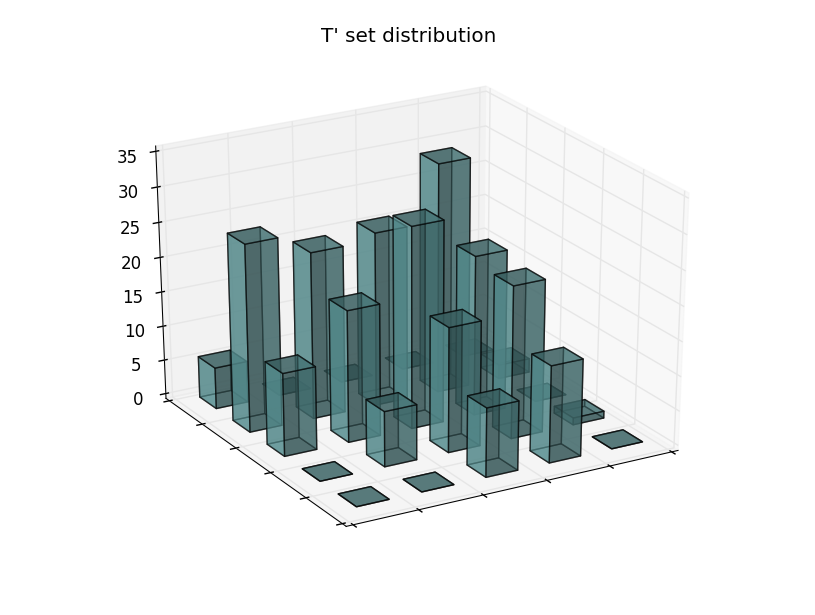
\includegraphics[height=10cm]{pic/fig6_mod2.png}
\caption{Выборка непересекающихся множеств для $n = 6$, подход 1}\label{fig2}
\end{figure}

Второй подход заключается

В результате выполнения алгоритма, гарантируется, что на выходе получится множество строк без повторов. 
При объединении полученного множества $T$ и получившихся на первом этапе строк, итоговое множетсво не превышает $2\cdot2^n$. 
Таким образом получается следующее распределение для $n = 6$, при этом размер множества составлял 124 строки. 

\begin{figure}[H]
\centering
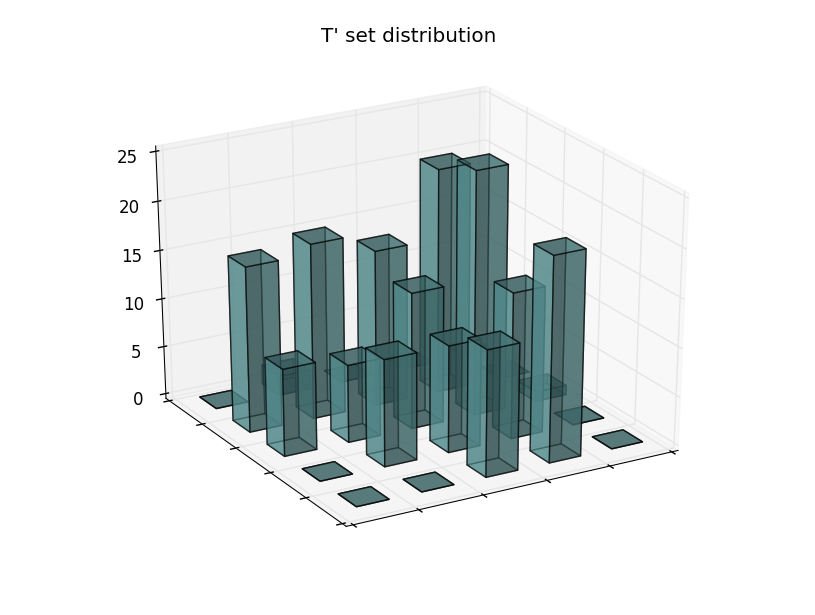
\includegraphics[height=10cm]{pic/fig6_mod3.png}
\caption{Выборка непересекающихся множеств для n = 6, подход 2}\label{fig2}
\end{figure}

В результате вызыва алгоритма для особей маленьких размеров, было замечено, что размер множества с повторами от увеличения размера особи растет экспоненциально. В таблице представлены результаты запуска для некоторых векторов:

\begin{table}[!h]
\caption{Результаты работы алгоритма с бинарными операторами}\label{tab3:apx}
\centering
\begin{tabu}{|*{6}{X[c]|}}\hline
n & 3 & 4 & 5 & 6 & 7  \\
\hline
set size & 8 & 16 & 32 & 64 & 128 \\
\hline
{T' size} & 64 & 256 & 1024 & 4096 & 16384  \\
\hline
{mod(T') size} & 11 & 36 & 73 & 144 & 302  \\
\hline
\end{tabu}
\end{table}

Ниже на рисунке~\ref{fig3} приводится диаграмма по количеству полученных совпавших строк и количеству оставшихся после модификации (берется лучшее значение).

\begin{figure}[H]
\centering
\caption{Выборка непересекающихся множеств для $n = 6$, подход 2}\label{fig3}
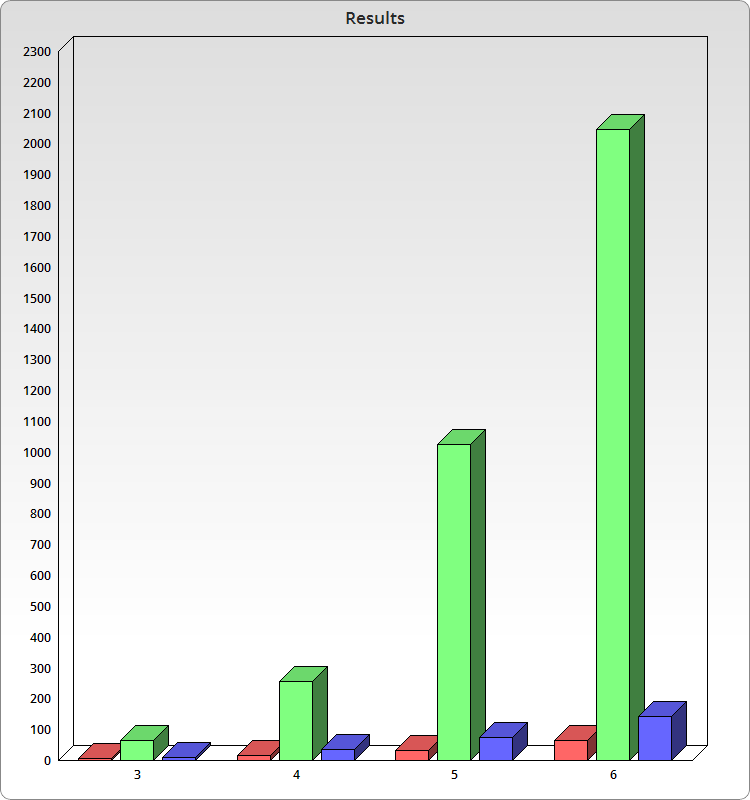
\includegraphics[height=10cm]{pic/res_bin.png}
\end{figure}


\subsection{Унарный алгоритм}
\label{unary}

%описание оператора и принципа
В силу того, что унарный несмещенный оператор может изменять только один случайный бит в векторе, в модели генетических алгоритмов он представляет собой оператор мутации. 

(Не хватает немного)

Разобъем все пространство поиска на некоторые классы векторов, где каждый шаг - это расстояние между первоначальным вектором и векторами этого множетсва, то есть, количество отличающихся бит. Классы будут генерироваться слеующим образом: 
\begin{itemize}
   \item $q_0$ $\leftarrow$ random
   \item $D_1$ - класс решений, отличающихся от первоначальной особи на 1 бит, размер множества n
   \item $D_2$ - размер ${n}\choose{2}$
   \item $D_3$ ...
   \item ...
   \item $D_{n-1}$ - размер ${n}\choose{n - 1}$ = n
   \item $D_n$ - размер 1, \bar{q_0}
\end{itemize} 


\newtheorem{theorem}{Теорема}
\begin{myth}
Даны непересекающиеся множества $S_1, ... S_k$ размеров $n_1 ... n_k$.
В одном из множеств находится элемент x. Утверждается, что в этой постановке при отсутствии другой информации, оптимизационный алгоритм выглядит так: 
\begin{algorithm}[H]
\caption{Унарный алгоритм}\label{lst1}
\begin{algorithmic}
        \For{i = 0, ... , k}
	    \State Храним $t_1 ... t_k$ - сколько запросов было сделано к соответствующему множеству
	    \State На определенном шаге вычисляем $E[z_i] = (\frac{n_i - 1}{n_i})^{t_i}$
	    \State Выбираем множество i c максимальным $E[z_i]$ и делаем запрос к этому множеству.
	    \EndFor
\end{algorithmic}
\end{algorithm}
\end{myth}
\begin{proof}
    Пусть мы знаем, сколько уникальных элементов $u_1...u_k$ было запрошено из каждого множества. Известно что количество элементов будет меньше или равно числу запросов к множеству. ($u_i \leq t_i$). 
    
    Пусть x - искомый экземпляр данной задачи, находится соответственно в одном из множеств. Предположим, что элемент x раньше не возвращался из запросов (так как при возвращении искомого элемента функция бы завершилась).
    
    
    $P_i$ = [вероятность, что $x$ лежит в $i$] = $\frac{t_i - u_i}{\sum_{j}{t_j - u_j}}$ 
    
    $p_i$ = [вероятность, что на запросе к i вернут k] = $\frac{1}{n_i} \cdot P_i$ = $\frac{n_i - u_i}{\sum_{j}{t_j - u_j}}$
    
    Так как $u_i$ - величина переменная а каждом шаге, можем посчитать матожидание в таком формате: $u_i \sim E(u_i(n_i, t_i))$
    
    До запроса было x уникальных запросов, после запроса будет: $$x + \frac{n - x}{n} = 1 + x \cdot (1 - \frac{1}{n_i})$$ 
    
    Таким образом: $E[u(n_i, t_i)] = 1 + E[u_i(n_i, t_{i} - 1)] \cdot (1 - \frac{1}{n_i})$
    
    Для $ t_i = 0 \to 0 $ - база индукции.
    
    Рассмотрим переход: 
    $E[u(n_i, t_i)]$ = $\frac{{n_i}^{ti} - {(n_i - 1)}^{ti}}{{n_i}^{t_i - 1}}$  = 1 + $[ \frac{{n_i}^{ti} - {(n_i - 1)}^{t_i}}{{n_i}^{t_i}} ] \cdot (\frac{1}{n_i})$ = $ \frac{{n_i}^{ti + 1} - {(n_i - 1)}^{t_i + 1}}{{n_i}^{t_i}} $ 
    
    Таким образом мы получаем значение, равное количеству строк на следующем шагу, а значит, теорема доказана.

\end{proof}

%здесь будет вставка от Дена для увеличения объема работы. Не знаю, пригодится ли дальше это, но пока пусть будет.

(доделать доказательство, доделать разбор вероятностей по классам)


\chapterconclusion

В этой главе представлены алгоритмы решения задачи Needle, использующие несмещенные операторы, а также информационно-теоретические оценки времени работы данных алгоритмов. Были рассмотрены 
унарные, бинарные и тернарные несмещенные операторы. Основной вывод главы заключается в получении верхних оценок на операторы арностей $k = 1, 2, 3$, а так же получение того, что нижняя и верхняя оценка 
работы тернарного алгоритма совпадают.
